\documentclass[12pt]{article}

\usepackage{amsmath}
\usepackage{amssymb}
\usepackage{graphicx}

\counterwithin*{equation}{section}
\counterwithin*{equation}{subsection}

\graphicspath{ {./images/} } 

\begin{document}
\section{Equations of Lines and Planes} 

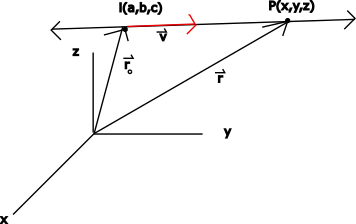
\includegraphics{line3d}
\fbox{$\vec{r} =\vec{r_0} +t \vec{v} $}

$t$ is the paramater of the equation.

Reiterate: $\vec{r} = \vec{r_0} +t \vec{iP} $

Let $\vec{v}=<a,b,c> $\\%
then $<x,y,z>=<x_0,y_0,z_0> + t<a,b,c>$\\%
$<x,y,z>=<x_0+ta,y_0+tb, z_0+tc>$

So the parametric equations for a line are as follows:
\begin{itemize}
	\item $x=x_0+ta$
	\item $y=y_0+tb$
	\item $z=z_0+tc$
\end{itemize}

When you solve for $t$, you get the \underline{symmetric equations}.\\%
$t=\frac{x-x_0}{a}=\frac{y-y_0}{b}=\frac{z-z_0}{c}$

If $b=0$, then you get:\\%
$\frac{x-x_0}{a}=\frac{z-z_0}{c}, y=y_0$



\textbf{incomplete do later}

Ex. 
Find where line L intersects plane $5x-2y+4z=18$

$L: x= -4t,\ y=5+t,\ z=2+3t$
\begin{align}
5(-4t)-2(5+t)+4(2+3t)=18\\
-20t-10-2t+8+12t=18\\
-10t=20\\
t=-2
\end{align}.
\begin{enumerate}
	\item Two planes are parallel if their normal vectors are parallel.
	\item Two planes that are not parallel intersect along a line
	\item The angle between intersecting planes is the angle between their normal vectors 
\end{enumerate}

Ex.: Consider planes $x+y+z=1$ and $3x+y-2z=1$

a) Find the angle between the planes
\subsection{Continued}
\begin{align}
	\vec{n_1}=<1,1,1>,\vec{n_2}=<3,1,-2> \\%
	\vec{n_1} \cdot {\vec{n_2}}=|\vec{n_1}||\vec{n_2}|\cos\theta 
\end{align}
Use the equations of two planes to describe a line\\%
Distance from a point to a plane\\%
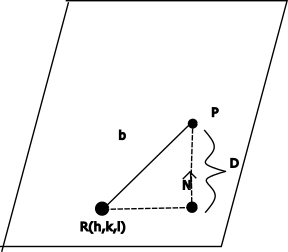
\includegraphics{ramppbn}\\%
$P_1(x_1,y_1,z_1)$\\%
$ax+by+cz+d=0$


EX: Find the distance between the parallel planes

\subsection
Ex: Find the distance between the lines $L_1$ and $L_2$ 

The distance between $L_1$ and $L_2$ is teh same as teh distance between the two parallel planes that contain these lines.\\
The normal vector $\vec{n}$ for these two planes must be orthogonal to $\vec{v_1}$ and $\vec{v_2}$
\end{document}


